\section{Закон сохранения энергии}

\begin{wrapfigure}{r}{2.5cm}
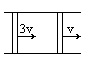
\includegraphics[scale=1]{0901LawOfConservationOfEnergyTwoPistons.jpg}
\end{wrapfigure}

%1
\AddProb В длинной теплоизолированной трубке между одинаковыми поршнями массы $m$ находится 1 моль одноатомного идеального газа при температуре $T_0$. 
В начальный момент скорости поршней направлены в одну сторону и равны $v$ и $3v$. До какой максимальной температуры нагреется газ? 
Поршни тепло не проводят, массой газа по сравнению с массой поршней пренебречь.

\AddProb (2004) В длинной горизонтальной трубе могут скользить без трения два поршня, массы которых $m$ и $2m$. 
Между ними находится некоторое количество одноатомного газа при давлении $p$ и объеме $V$. 
В этот момент легкий поршень движется к тяжелому со скоростью $v_0$, тяжелый поршень покоится. 
Оцените максимальную скорость тяжелого поршня.

\AddProb (2003) Внутри закрытого теплоизолированного цилиндра с идеальным газом находится легкоподвижный теплопроводящий поршень. 
При равновесии поршень делит цилиндр на две равные части и температура газа равна $T_0$. Поршень начали медленно перемещать. 
Найти температуру газа как функцию отношения $\eta$ объема большей части к объему меньшей части. Показатель адиабаты газа~$\gamma$.

\begin{wrapfigure}{r}{3cm}
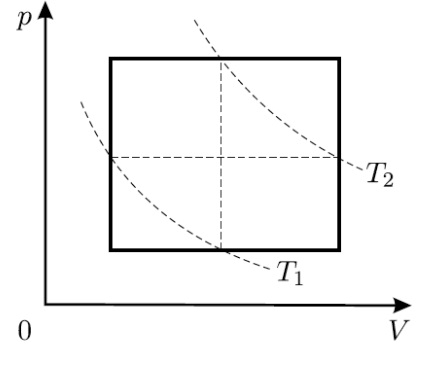
\includegraphics[scale=0.25]{0904LawOfConservationOfEnergyEfficiency.jpg}
\end{wrapfigure}

\AddProb Найдите КПД тепловой машины, цикл которой состоит из двух изохор и двух изобар, а рабочим телом является идеальный одноатомный газ. 
Середины нижней изобары и левой изохоры лежат на изотерме, соответствующей температуре $T_1$, 
а середины верхней изобары и правой изохоры -- на изотерме, соответствующей температуре~$T_2$.

\AddProb (2014) В вертикальном цилиндрическом сосуде с теплонепроницаемыми стенками под поршнем массы $m$~=~100~г находится 5 моль неона 
(молярная масса 20 г/моль). В начальный момент поршень закреплен. После того, как поршень освободили, объем газа увеличился в 2 раза. 
Определите конечную температуру газа, если его начальная температура равна $T_0$ = 300~К. Считайте, что над поршнем вакуум. 
Трением между поршнем и стенками сосуда отсутствует.

\begin{wrapfigure}{r}{3cm}
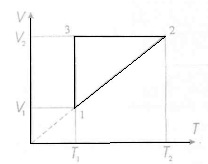
\includegraphics[width=3cm]{092002LawOfConservationOfEnergyProcess.jpg}
\end{wrapfigure}

%6
\AddProb (2002) Чему равна работа 1 моля идеального газа в круговом процессе, показанном на рисунке? Температуры $T_1$ и $T_2$ известны.

\section{Теплоемкость}

\AddProb (1998) Имеется идеальный газ, теплоемкость которого при постоянном объеме равна $C_V$. 
Найдите молярную теплоемкость этого газа как функцию объема, если давление газа меняется по закону $p=p_0~e^{\alpha V}$ ($p_0$ и $\alpha$ известны).

\AddProb Найдите максимальную температуру идеального газа в процессе, протекающем по закону $P=P_0~-~\alpha~V^2$, 
где $P_0$ и $\alpha$ -- положительные постоянные, $V$ -- объем одного моля.

\AddProb Для идеального газа с заданным показателем адиабаты $\gamma$ найдите уравнение процесса (в координатах $V$, $T$), 
при котором теплоемкость зависит от температуры по закону $c=\xi~T^2$.

\begin{wrapfigure}{r}{4cm}
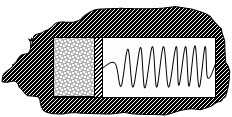
\includegraphics[scale=0.6]{092005HeatCapacityCylinder.jpg}
\end{wrapfigure}

\AddProb (2005) В расположенном горизонтально цилиндре слева от закрепленного поршня находится один моль идеального газа, 
в правой части цилиндра - вакуум. Цилиндр теплоизолирован от окружающей среды, а пружина, расположенная между поршнем и стенкой, 
находится первоначально в недеформированном состоянии. Поршень освобождают, и после установления равновесия объем, занимаемый газом, 
увеличивается в $\alpha$ раз. Как изменились при этом температура и давление газа? Теплоемкостями цилиндра, поршня и пружины пренебречь. 
Найти теплоемкость газа.

\begin{wrapfigure}{r}{3cm}
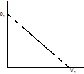
\includegraphics{082001GasLawsProcess.jpg}
\end{wrapfigure}

%11
\AddProb (2001) Вычислить молярную теплоемкость $C_P(V)$ идеального газа, совершающего процесс, показанный на рисунке. 
Показатель адиабаты $\gamma$ считать известным.